%%%%%%%%%%%%%%%%%%%%%%%%%%%%%%%%%%%%%%%%%%%%%%%%%%%%%%%%%%%%%%%%%%%%%%
% How to use writeLaTeX: 
%
% You edit the source code here on the left, and the preview on the
% right shows you the result within a few seconds.
%
% Bookmark this page and share the URL with your co-authors. They can
% edit at the same time!
%
% You can upload figures, bibliographies, custom classes and
% styles using the files menu.
%
%%%%%%%%%%%%%%%%%%%%%%%%%%%%%%%%%%%%%%%%%%%%%%%%%%%%%%%%%%%%%%%%%%%%%%

\documentclass[12pt]{article}

\usepackage{assets/helpers/sbc-template}
\usepackage{graphicx,url}
\usepackage[brazil]{babel}   
\usepackage[utf8]{inputenc}  

\sloppy

\title{Instructions for Authors of SBC Conferences\\ Papers and Abstracts}

\author{Isabella de Freitas Nunes\inst{1}}


\address{Universidade do Vale do Itajaí
  (Univali)\\
  Rua Uruguai, 458 - Centro - Itajaí - Santa Catarina - Brasil - 88302-901
  \email{R.Bordini@durham.ac.uk}
}

\begin{document} 

\maketitle

\begin{abstract}
  This article describes the building of an IoT system implemented using an ESP8266 microcontroller with FreeRTOS framework. The system uses a DHT11 sensor for temperature and humidity monitoring, then MQTT protocol is used to transmit collected data to a broker. The solution includes Wi-Fi management, real-time status monitoring, and fault tolerance to maintain reliability in data acquisition and transmission. Also a local Frontend was developed using React, to use the data sent to the broker.
\end{abstract}
     
\begin{resumo} 
  Este artigo descreve a construção de um sistema de IoT implementado utilizando um microcontrolador ESP8266 com o framework FreeRTOS. O sistema usa um sensor DHT11 para monitoramento de temperatura e umidade e, em seguida, o protocolo MQTT é usado para transmitir os dados coletados a um broker. A solução inclui gerenciamento de Wi-Fi, monitoramento de status em tempo real e tolerância a falhas para manter a confiabilidade na aquisição e transmissão de dados. Também foi desenvolvido um Frontend local utilizando React, para utilizar os dados enviados ao corretor.
\end{resumo}

\section{General Information}
\section{First Page} \label{sec:firstpage}
\section{CD-ROMs and Printed Proceedings}
\section{Sections and Paragraphs}
\subsection{Subsections}
\section{Figures and Captions}\label{sec:figs}
\begin{figure}[ht]
\centering
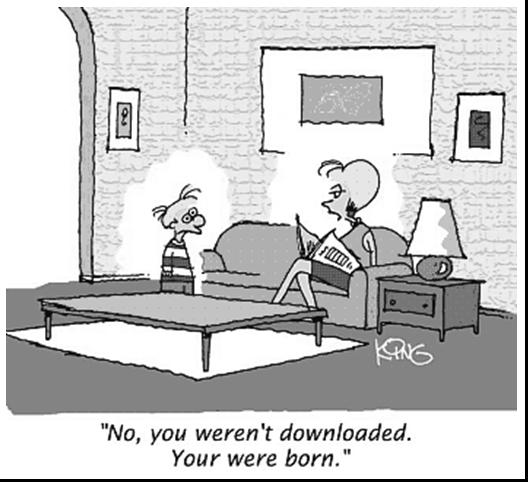
\includegraphics[width=.5\textwidth]{assets/img/fig1.jpg}
\caption{A typical figure}
\label{fig:exampleFig1}
\end{figure}

\begin{figure}[ht]
\centering
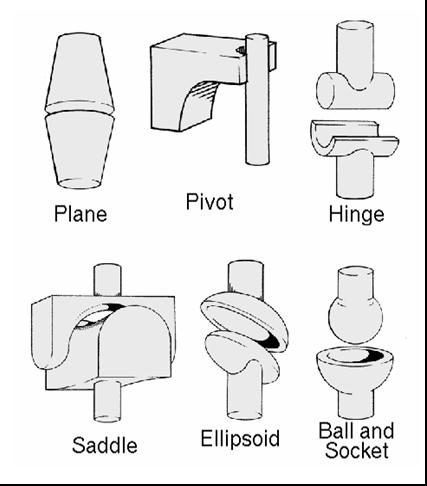
\includegraphics[width=.3\textwidth]{assets/img/fig2.jpg}
\caption{This figure is an example of a figure caption taking more than one
  line and justified considering margins mentioned in Section~\ref{sec:figs}.}
\label{fig:exampleFig2}
\end{figure}
\begin{table}[ht]
\centering
\caption{Variables to be considered on the evaluation of interaction
  techniques}
\label{tab:exTable1}
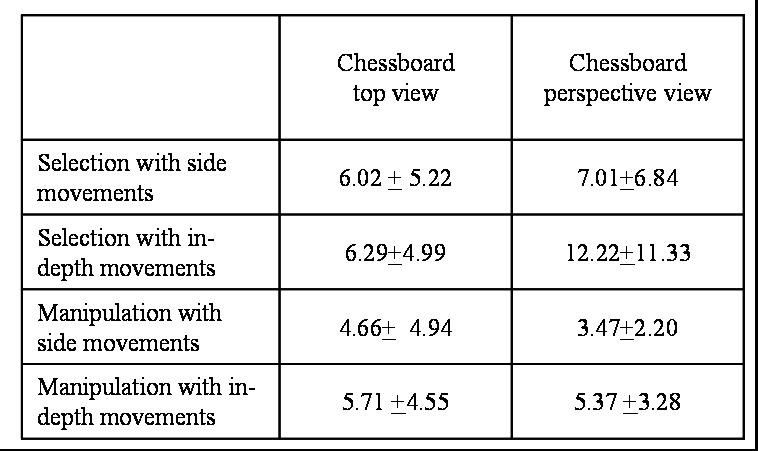
\includegraphics[width=.7\textwidth]{assets/img/table.jpg}
\end{table}
\section{Images}

\bibliographystyle{assets/helpers/sbc}
\bibliography{assets/helpers/sbc-template}

\end{document}
